\section{Checkpoint 3}

\addtocounter{subsection}{1}

\subsection{What is a Programm? What is a Process? What is a Thread?}
Ein Programm ist eine ausf\"uhrbare Datei.\\
Ein Prozess ist ein laufendes Programm.\\
Ein Thread ist ein Ausf\"uhrungsstrang eines Programms.

\subsection{What are the roles of the scheduler and the dispatcher?}
Der Scheduler hat die Aufgabe den laufenden Prozessen ihre CPU Zeit zuzuweisen.\\
Der Dispatcher gibt die Kontrolle zum dem n\"achsten aktiven Thread(wiederherstellen des CPU Kontextes, vorbereiten des Adressbereiches f\"ur den n\"achsten Prozess).

\subsection{Compare the long term scheduler to the short term scheduler.}
Long-term scheduler(Steuert Grad der Multiprogrammierung, kann Prozesse schlafen legen, optional)\\
Short-term scheduler(Sucht zu jedem Quantum einen neuen Thread aus, Scheduler \"uber den wir immer reden)

\subsection{Describe 3 properties related to process and thread control objects.}
\begin{itemize}
	\item Prozess: Speicherbereich, Pfad der ausf\"uhrbaren Datei
	\item Thread: CPU Kontext, Schedulingzustand
	\item Beides: Nicewert(Priorit\"aten), ID
\end{itemize}

\subsection{Describe 3 properties related to the CPU context.}
Prozessorstatuswort, Stackregister, Datenregister, Programmcounter

\subsection{Outline the sequence of a context switch as performed by the dispatcher.}
Aktuellen Thread unterbrechen $\rightarrow$ Aktuellen Zustand sichern im Hauptspeicher $\rightarrow$ Daten vom anderen Thread zur\"uckschreiben $\rightarrow$ anderen Thread ausf\"uhren

\subsection{Compare cooperative to preemptive scheduling.}
\textbf{cooperative} freiwillige Abgabe der CPU\\
\textbf{preemptive} Unterbrechung, wenn Quantum abgelaufen

\subsection{What is a quantum? What effect does the length of a quantum have on the scheduler performance?}
Ein Quantum ist eine feste Zeitscheibe, welche angibt wie lange ein Prozess rechnen darf, bis er unterbrochen wird. L\"angeres Quantum sorgt f\"ur eine h\"ohere Performanz. K\"urzeres Quantum ist responsiver.

\subsection{Threads can have different states in relation to scheduling. Draw a diagram and Describe the purpose of the states and their transitions.}

\begin{figure}[H]
	\centering
	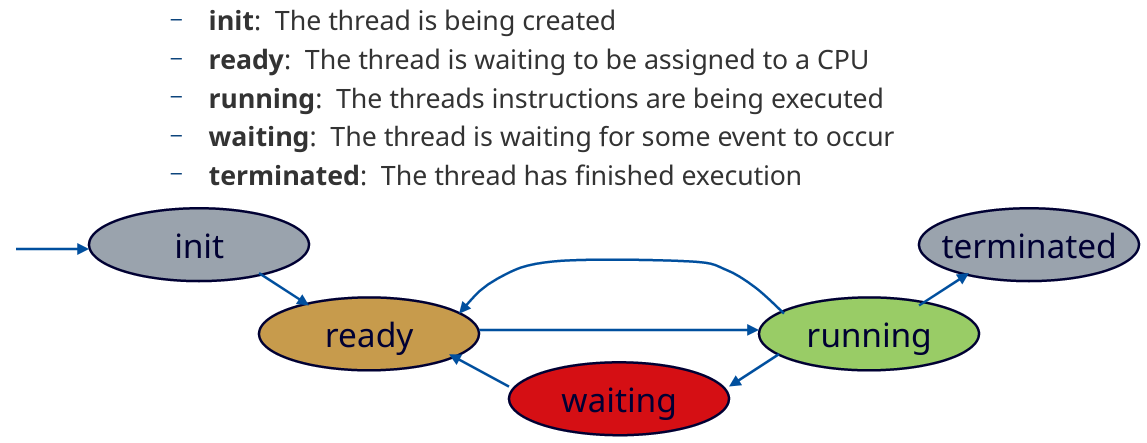
\includegraphics[width=0.7\linewidth]{Pictures/scheduling_dia}
	\caption{bla}
	\label{fig:schema01}
\end{figure}

\subsection{When are scheduling decisions made?}